\documentclass[12pt]{article}
\usepackage{setspace}
\usepackage{amsmath}
\usepackage[utf8]{inputenc}
\usepackage{pgfplots}
\pgfplotsset{compat=1.16}
\usepgfplotslibrary{statistics}


\oddsidemargin=0.0in
\evensidemargin=0.0in
\textwidth=6.5in
\headheight=0.0in
\topmargin=0.0in
\textheight=9.5in
\title{Minimising Portfolio Loss in Portfolio Construction}
%\date{16-12-2021}
\author{Colin M. Smith BITA Risk}
\begin{document}
\maketitle
\tableofcontents
\pagebreak
\doublespacing
\section{Introduction}
This document attempts to show how to use portfolio loss minimisation in the
portfolio enhancement process. We start by defining $Loss$ and compare
the predicted changes to a portfolio given by minimal $Loss$ and minimal $Risk$.
\section{Definition of Portfolio Gain and Loss}
Over the history of a portfolio it is usual to monitor its return each period and the returns of the underlying assets.
From one period  to the next, the portfolio's return will change and to characterise this change we can define its gain or loss.
To make the gain and loss a little more configurable we define 
gain $G$ and loss $L$ with respect to a target return $R$ which could be positive or negative.
Suppose the portfolio return series at time $t$ is $r(t)$ then
\begin{eqnarray}
    G = \sum_t {\textbf{ max} }(r(t) - R,0)
\end{eqnarray}
\begin{eqnarray}
    L = \sum_t {\textbf{ max} }(R-r(t),0)
\end{eqnarray}
This means that in period $t$, if $R-r(t) > 0$ there is a loss, and if $R-r(t) < 0$ there is a gain.
If we define a loss period as one for which $R-r(t) > 0$,
\begin{eqnarray}
  {\rm Total\ Loss},\ L= \sum_{t\ \in\ \rm loss\ periods} R-r(t)
\end{eqnarray}
$G$ and $L$ are both non-negative and
\begin{eqnarray}
 {\rm   total\ portfolio\ return}= G - L + RT
\end{eqnarray}

If there are $n$ assets in the portfolio and each asset $i$
has a weight $w_i$ and a return series $s_i (t)$ then
\begin{eqnarray}
    r(t) = \sum_{i=1}^{n} w_i s_i(t)
\end{eqnarray}
The expected return for asset $i$, $\alpha_i$ may be calculated from
mean\footnote{We calculate $\alpha$ using arithmetic mean. $\alpha_i$ and target rate are values per-period.} 
return of $s_i(t)$.
\begin{eqnarray}
    \alpha_i =  \frac{1}{T}\sum_{t=1}^{T} s_i(t)
\end{eqnarray}
where $T$ is the number of periods.
\section{Comparison of Optimal Portfolio Weights in Risk and Loss Minimisation}
In a standard portfolio construction exercise we seek to find a portfolio that will 
give a certain amount of return for minimum risk. As well as this we could also do a 
different optimisation and fix the 
return but find the lowest possible loss. Consider a small portfolio of 9 assets.
The following graph shows the outcome weights for two portfolio optimisations. In both the return is 
constrained to $0.005$ and the target rate per period is $0.0004$; the blue bars show the weights
for mininum risk ($0.058$) which has a loss of $1.34$ and the pink bars show
the weights for minimum loss ($1.15$) with a risk of $0.085$. The risk quoted here is historic risk 
calculated directly as standard deviation of portfolio return series.

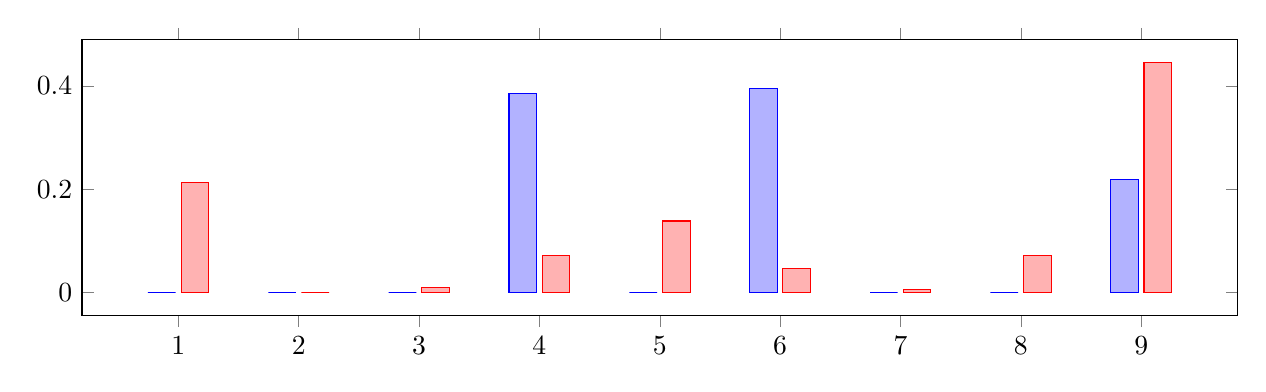
\begin{tikzpicture}
    \begin{axis}
        [ybar,height=2in,width=6.4in, symbolic x coords={1,2,3,4,5,6,7,8,9}]
        \addplot+ coordinates {(1,0)
        (2,0) 
        (3,0)
        (4,0.3854726513396513)
        (5,0)
        (6,0.3950537500804109)
        (7,0)
        (8,0)
        (9,0.21947359857993776)};
        \addplot+ coordinates {
            (1,0.2131871336385196)
            (2,0)
            (3,0.008529985052857314)
            (4,0.07179520200177866)
            (5,0.13819750244263093)
            (6,0.046937456187809756)
            (7,0.0047705423361060345)
            (8,0.07143877895977421)
            (9,0.4451433993805218)};
    \end{axis}
\end{tikzpicture}

If we just maximised return the portfolio would have all weight in the last 
asset and the return would be $0.0098$.

\section{Minimising Loss in the Enhancements}
The driving force in the portfolio enhancement process could be the imposition
of factor constraints. There are many other restrictions going on, but the main one for 
achieving extra portfolio return is due to the factor premia constraints. A straightforward 
implementation of loss optimisation might be to replace the risk optimisation with loss minimisation.
Typically this would be done using full asset return history to define $Loss$ and could 
result in a slow optimisation process since the amount of history is so vast. (It would be possible 
to use a risk constraint as well but this would mean even longer execution time.) The advantage of
minimising $Loss$ over minimising $Risk$ is that the resulting weights are likely
to be more diversifing. Looking at the simple graph for 9 stocks in the previous section we see that
$Loss$ minimisation results in higher weight in the high alpha asset with many 
smaller changes in the other assets to get the loweest loss. ($Risk$ optimisation gives a less diverse
result and a lower weight in the high alpha asset). We conjecture from this that $Loss$ minimisation 
would make less impact on the strength of the factor premia terms, than $Risk$ minimisation. 

The difference in weight outcomes also
highlights that the gains and losses in the optimisation are not symmetrically
distributed. If they were, minimising $Loss$ would be very similar to minimising historic $Risk$, (although
we do impose our own asymmetricity by having a non-zero tartget rate.) It is important
to note that the factor premia must not be constrained too high, otherwise there is no scope 
for miminising $Loss$ (or $Risk$ either). In the example in the previous section 
if we had constrained the return to be $0.0098$ the only possible outcome has $100\%$ in 
the last asset.
\section{Minimising Modelled Loss}
The calculation outlined in the previous might be thought as $`$traditional gain loss'; it
minimises historic $loss$ subject to all of the portfolio constraints. Usually the risk in 
portfolio enhancement is modelled risk; it might be better to use modelled $Loss$ here.

The risk model estimation process uses factor premia returns in the regression
with asset returns. If there are $n_f$ factor premia, the modelled asset return $\hat{r}_{k}$ for asset $k$ may be written
\begin{eqnarray}
    \hat{r}_{k}(t) = \sum_{i=1}^{i=n_f}\beta_{ki} p_{i}(t)
\end{eqnarray}
at time $t$, where $p_i$ is the i'th factor return and $\beta$ is the usual factor loading, regression coefficient.
Due to cycle conditions a 3 month forecast window\footnote{One month would be too short an estimation period.} of factor premia data may be enough
to get a good prediction of future return, so instead of incorporating the full history of
asset returns $r_k(t)$ in the optimisation it may be enough to use the modelled predictions
$\hat{r}_{k}(t)$ over a much reduced time horizon. The shorter the history for defining the
loss, the faster the optimisation, so there is a practical reason for this as well as
a theoretical one.
\end{document}

